%% ============================================================
%%  PARTE 2 — Estudio experimental CEC2017
%%  Hasta 1.5 puntos
%% ============================================================

\newpage
\section{Parte II: Estudio Experimental sobre CEC2017}
\label{sec:parte2}

\subsection{Configuración experimental}

El estudio experimental sigue las condiciones estándar del benchmark CEC2017
\cite{wu2016cec2017}, cuyo objetivo es comparar metaheurísticas de manera justa
e imparcial sobre funciones de prueba de optimización continua.

\begin{table}[h!]
\centering
\caption{Condiciones experimentales del estudio sobre CEC2017}
\label{tab:config}
\renewcommand{\arraystretch}{1.3}
\small
\begin{tabular}{@{}ll@{}}
\toprule
\textbf{Parámetro} & \textbf{Valor} \\
\midrule
Número de funciones & 30 (F1--F30; unimodales, multimodales, híbridas y compuestas) \\
Dimensiones & $D \in \{10, 30, 50\}$ \\
Evaluaciones máximas & $10{,}000 \times D$ \\
Rango de búsqueda & $[-100, 100]^D$ \\
Número de ejecuciones & 31 ejecuciones independientes (semillas $1,2,\ldots,31$) \\
Métrica & Error respecto al óptimo conocido: $f(\mathbf{x}) - f(\mathbf{x}^*)$ \\
Puntos de registro & 1\%, 2\%, 3\%, 5\%, 10\%, 20\%, \ldots, 100\% de las evaluaciones \\
\bottomrule
\end{tabular}
\end{table}

\subsubsection{Parámetros del LCA}

Los parámetros del LCA base utilizados en el estudio experimental son:

\begin{table}[h!]
\centering
\caption{Configuración de parámetros del LCA para CEC2017}
\label{tab:params_lca}
\renewcommand{\arraystretch}{1.3}
\footnotesize
\begin{tabular}{@{}lll@{}}
\toprule
\textbf{Parámetro} & \textbf{Valor} & \textbf{Descripción} \\
\midrule
$N$ & 30 & Tamaño de la población (número de tumores) \\
$\beta$ & 1.5 & Parámetro del vuelo de Lévy (Mantegna) \\
$\zeta$ & $t/T$ & Tasa de mutación adaptativa (crece linealmente) \\
$T$ & $\lfloor 10{,}000 \cdot D / (4N) \rfloor$ & Iteraciones máximas (4 evaluaciones por tumor e iteración) \\
$lb, ub$ & $-100, 100$ & Límites del espacio de búsqueda \\
\bottomrule
\end{tabular}
\end{table}

\subsection{Implementación del LCA sobre CEC2017}

El algoritmo LCA se ha implementado en \texttt{C++} utilizando la API del repositorio
\texttt{cec2017real} \cite{molina2017cec}. El núcleo del LCA (evaluación con control de
presupuesto, inicialización ROBL, fase de crecimiento/Lévy y operadores de metástasis) se
encuentra en el fichero \texttt{testlca.cc} del software entregado, siguiendo las ecuaciones
de la Parte~I.

Como algoritmos de referencia se han implementado igualmente, bajo el mismo protocolo
y la misma API de evaluación, dos metaheurísticas clásicas ampliamente validadas:
\textbf{Evolución Diferencial} (DE/rand/1/bin, con $F=0.5$, $CR=0.9$, $N=50$) \cite{storn1997de}
y \textbf{Optimización por Enjambre de Partículas} (PSO con coeficientes de constricción
$w=0.7298$, $c_1=c_2=1.49618$, $N=50$) \cite{kennedy1995pso}. De este modo, las tres
metaheurísticas comparten exactamente las mismas condiciones experimentales (presupuesto,
rango, semillas y número de ejecuciones), garantizando una comparación justa.

Se han elegido precisamente \textbf{DE} y \textbf{PSO} por ser los dos \emph{baselines}
canónicos de la optimización continua de caja negra: DE \cite{storn1997de} representa el
paradigma evolutivo basado en diferencias de vectores, y PSO \cite{kennedy1995pso} el
paradigma de inteligencia de enjambre. Ambos están sobradamente validados sobre CEC y
constituyen la referencia obligada para situar el rendimiento de cualquier metaheurística
nueva; superar (o no) a este par es la prueba estándar del estado del arte clásico.

\subsubsection{Desviaciones respecto a la formulación original}

La implementación aquí evaluada introduce, de forma deliberada, tres simplificaciones
respecto al algoritmo original de Houssein \emph{et al.} \cite{houssein2023lca}, que conviene
declarar explícitamente para una interpretación honesta de los resultados:

\begin{enumerate}
  \item \textbf{Selección de operador por probabilidad.} El paper calcula en cada iteración
    \emph{tanto} el crecimiento $y = \text{Position}+PG$ \emph{como} el salto de Lévy
    $Z = y + S\cdot LF$ y conserva el de mejor fitness (Eqs.~6--8). La implementación adopta
    en su lugar un \textbf{selector probabilístico}: con probabilidad $0.8$ aplica crecimiento
    y con $0.2$ aplica Lévy. Esto reduce a la mitad las evaluaciones por agente, pero limita
    el refinamiento local al prescindir de la comparación directa entre ambos movimientos.
  \item \textbf{Inicialización ROBL.} Se emplea la forma clásica de \emph{opposition-based
    learning} $x_{\text{opp}} = lb + ub - r\cdot x$ en lugar del término geométrico
    $(\pi/6)\,\ell\,w\,h$ de la Eq.~(1). Solo afecta a la población inicial.
  \item \textbf{Mutación.} El componente $y$ de la mutación (Eq.~10--12) incorpora un factor
    aleatorio adicional ($y = |\text{Position}-X_{\text{best}}|\cdot r$ frente a
    $y = |\text{Position}-X_{\text{best}}|$ del paper).
\end{enumerate}

Estas decisiones priorizan la simplicidad de implementación y un menor coste por iteración;
como se discute más adelante, contribuyen a la explotación local deficiente del LCA base y
motivan directamente la hibridación memética de la Parte~III.

\subsection{Resultados experimentales}

Los resultados se presentan como el \textbf{error medio} respecto al óptimo conocido
($f(\mathbf{x}) - f(\mathbf{x}^*)$) en el hito del 100\,\% del presupuesto
($10\,000 \times D$ evaluaciones), promediado sobre las \textbf{31 ejecuciones
independientes} (semillas $1$ a $31$). Se reportan las tres dimensiones $D \in \{10, 30, 50\}$.
Las funciones se agrupan según el protocolo CEC2017: F1--F3 unimodales, F4--F10 multimodales
simples, F11--F20 híbridas y F21--F30 compuestas.

\begin{table}[h!]
\centering
\caption{Error medio sobre CEC2017 ($D=10$, 31 ejecuciones). En negrita el mejor por función.}
\label{tab:res_d10}
\footnotesize
\renewcommand{\arraystretch}{1.1}
\begin{tabular}{@{}lrrr@{}}
\toprule
\textbf{Función} & \textbf{DE} & \textbf{LCA} & \textbf{PSO} \\
\midrule
F01 & \textbf{0.000e+00} & 2.122e+09 & 3.694e+03 \\
F02 & \textbf{0.000e+00} & 8.532e+06 & 1.291e+05 \\
F03 & \textbf{0.000e+00} & 8.545e+03 & 7.335e-15 \\
F04 & \textbf{4.967e-01} & 4.711e+01 & 1.515e+01 \\
F05 & \textbf{7.207e+00} & 4.475e+01 & 1.568e+01 \\
F06 & \textbf{0.000e+00} & 2.096e+01 & 3.911e-01 \\
F07 & \textbf{1.973e+01} & 5.959e+01 & 2.186e+01 \\
F08 & \textbf{6.809e+00} & 2.681e+01 & 1.207e+01 \\
F09 & \textbf{0.000e+00} & 1.527e+02 & 3.798e-02 \\
F10 & \textbf{3.532e+02} & 7.532e+02 & 5.513e+02 \\
F11 & \textbf{4.863e-01} & 7.481e+01 & 1.033e+01 \\
F12 & \textbf{6.439e+01} & 1.314e+06 & 4.374e+05 \\
F13 & \textbf{4.903e+00} & 3.787e+03 & 7.385e+03 \\
F14 & \textbf{6.419e-01} & 9.409e+01 & 5.340e+01 \\
F15 & \textbf{3.748e-01} & 3.260e+02 & 4.593e+01 \\
F16 & \textbf{5.124e+00} & 2.053e+02 & 1.543e+02 \\
F17 & \textbf{3.778e+00} & 6.503e+01 & 4.996e+01 \\
F18 & \textbf{2.107e+00} & 9.089e+03 & 1.210e+04 \\
F19 & \textbf{1.470e-01} & 8.656e+02 & 1.482e+02 \\
F20 & \textbf{3.159e-01} & 7.234e+01 & 7.513e+01 \\
F21 & \textbf{1.870e+02} & 1.979e+02 & 2.007e+02 \\
F22 & \textbf{9.705e+01} & 1.715e+02 & 1.069e+02 \\
F23 & \textbf{3.069e+02} & 3.615e+02 & 3.257e+02 \\
F24 & 3.289e+02 & \textbf{1.522e+02} & 3.336e+02 \\
F25 & \textbf{4.128e+02} & 4.994e+02 & 4.305e+02 \\
F26 & \textbf{3.435e+02} & 6.109e+02 & 4.072e+02 \\
F27 & \textbf{3.910e+02} & 4.144e+02 & 4.177e+02 \\
F28 & \textbf{4.228e+02} & 6.353e+02 & 5.291e+02 \\
F29 & \textbf{2.305e+02} & 3.271e+02 & 3.106e+02 \\
F30 & \textbf{7.718e+04} & 1.426e+05 & 2.823e+05 \\
\bottomrule
\end{tabular}
\end{table}

\begin{table}[h!]
\centering
\caption{Error medio sobre CEC2017 ($D=30$, 31 ejecuciones).}
\label{tab:res_d30}
\footnotesize
\renewcommand{\arraystretch}{1.1}
\begin{tabular}{@{}lrrr@{}}
\toprule
\textbf{Función} & \textbf{DE} & \textbf{LCA} & \textbf{PSO} \\
\midrule
F01 & \textbf{3.166e+03} & 1.665e+10 & 7.167e+08 \\
F02 & \textbf{1.082e+10} & 7.964e+33 & 3.023e+30 \\
F03 & 4.742e-04 & 6.203e+04 & \textbf{1.928e-09} \\
F04 & \textbf{5.294e+01} & 1.365e+03 & 2.070e+02 \\
F05 & \textbf{4.325e+01} & 2.476e+02 & 1.080e+02 \\
F06 & \textbf{9.400e-03} & 4.067e+01 & 8.681e+00 \\
F07 & 1.414e+02 & 4.576e+02 & \textbf{1.209e+02} \\
F08 & \textbf{4.812e+01} & 1.992e+02 & 9.992e+01 \\
F09 & \textbf{2.799e+00} & 3.514e+03 & 8.970e+02 \\
F10 & 4.418e+03 & 4.259e+03 & \textbf{3.472e+03} \\
F11 & \textbf{2.585e+01} & 2.103e+03 & 1.489e+02 \\
F12 & \textbf{1.673e+04} & 9.979e+08 & 6.081e+07 \\
F13 & \textbf{2.116e+02} & 2.223e+08 & 4.171e+07 \\
F14 & \textbf{2.814e+01} & 2.390e+05 & 1.770e+04 \\
F15 & \textbf{1.348e+01} & 1.351e+06 & 1.192e+04 \\
F16 & \textbf{3.941e+02} & 1.655e+03 & 1.044e+03 \\
F17 & \textbf{8.977e+01} & 6.203e+02 & 4.917e+02 \\
F18 & \textbf{1.297e+03} & 1.351e+06 & 1.203e+05 \\
F19 & \textbf{6.567e+00} & 2.913e+05 & 2.221e+04 \\
F20 & \textbf{1.024e+02} & 4.059e+02 & 3.920e+02 \\
F21 & \textbf{2.597e+02} & 3.545e+02 & 3.071e+02 \\
F22 & 2.401e+03 & 2.325e+03 & \textbf{2.036e+03} \\
F23 & \textbf{3.764e+02} & 6.712e+02 & 5.801e+02 \\
F24 & \textbf{4.562e+02} & 8.069e+02 & 6.613e+02 \\
F25 & \textbf{3.870e+02} & 6.517e+02 & 3.994e+02 \\
F26 & \textbf{1.249e+03} & 3.361e+03 & 2.214e+03 \\
F27 & \textbf{5.045e+02} & 6.129e+02 & 5.999e+02 \\
F28 & \textbf{3.834e+02} & 1.247e+03 & 5.178e+02 \\
F29 & \textbf{4.568e+02} & 1.458e+03 & 1.097e+03 \\
F30 & \textbf{2.261e+03} & 3.574e+07 & 5.020e+04 \\
\bottomrule
\end{tabular}
\end{table}

\begin{table}[h!]
\centering
\caption{Error medio sobre CEC2017 ($D=50$, 31 ejecuciones).}
\label{tab:res_d50}
\footnotesize
\renewcommand{\arraystretch}{1.1}
\begin{tabular}{@{}lrrr@{}}
\toprule
\textbf{Función} & \textbf{DE} & \textbf{LCA} & \textbf{PSO} \\
\midrule
F01 & \textbf{5.795e+03} & 4.782e+10 & 2.491e+09 \\
F02 & \textbf{3.887e+16} & 3.209e+56 & 7.526e+63 \\
F03 & 5.467e+03 & 1.309e+05 & \textbf{1.370e+03} \\
F04 & \textbf{8.139e+01} & 5.528e+03 & 4.671e+02 \\
F05 & \textbf{6.616e+01} & 4.013e+02 & 2.472e+02 \\
F06 & \textbf{2.913e-02} & 5.099e+01 & 2.728e+01 \\
F07 & \textbf{2.431e+02} & 9.124e+02 & 2.763e+02 \\
F08 & \textbf{6.262e+01} & 4.550e+02 & 2.391e+02 \\
F09 & \textbf{2.155e+01} & 1.113e+04 & 4.857e+03 \\
F10 & 1.130e+04 & 7.413e+03 & \textbf{6.198e+03} \\
F11 & \textbf{5.268e+01} & 8.602e+03 & 2.751e+02 \\
F12 & \textbf{9.561e+04} & 1.264e+10 & 2.239e+09 \\
F13 & \textbf{7.747e+03} & 4.351e+09 & 4.379e+08 \\
F14 & \textbf{8.578e+02} & 1.935e+06 & 1.184e+06 \\
F15 & \textbf{4.231e+03} & 5.119e+08 & 2.312e+06 \\
F16 & \textbf{1.282e+03} & 3.287e+03 & 1.722e+03 \\
F17 & \textbf{9.602e+02} & 2.033e+03 & 1.503e+03 \\
F18 & \textbf{8.079e+03} & 2.556e+07 & 3.787e+05 \\
F19 & \textbf{1.661e+03} & 5.326e+07 & 1.211e+06 \\
F20 & \textbf{8.857e+02} & 9.712e+02 & 1.089e+03 \\
F21 & \textbf{2.783e+02} & 6.086e+02 & 4.471e+02 \\
F22 & 1.315e+04 & 8.520e+03 & \textbf{7.073e+03} \\
F23 & \textbf{4.828e+02} & 1.124e+03 & 9.939e+02 \\
F24 & \textbf{6.066e+02} & 1.253e+03 & 1.101e+03 \\
F25 & \textbf{5.347e+02} & 2.681e+03 & 6.393e+02 \\
F26 & \textbf{1.708e+03} & 9.114e+03 & 4.027e+03 \\
F27 & \textbf{6.324e+02} & 1.144e+03 & 9.799e+02 \\
F28 & \textbf{4.901e+02} & 3.970e+03 & 8.984e+02 \\
F29 & \textbf{4.688e+02} & 3.071e+03 & 1.721e+03 \\
F30 & \textbf{6.563e+05} & 2.989e+08 & 3.872e+06 \\
\bottomrule
\end{tabular}
\end{table}

\subsection{Análisis estadístico no paramétrico}

Para validar las diferencias de rendimiento se sigue la metodología no paramétrica
habitual en este tipo de estudios, popularizada por la herramienta \textbf{Tacolab}
\cite{tacolab}: ranking medio de Friedman y test de Wilcoxon de rango con signo.
Dado que el análisis cubre las tres dimensiones y 31 ejecuciones, los estadísticos se han
calculado de forma reproducible con un script propio (\texttt{analysis.py}) sobre los
ficheros de resultados, replicando los tests que ofrece Tacolab.

\paragraph{¿Por qué tests no paramétricos?}
Los tests paramétricos clásicos (t de Student, ANOVA) exigen que los datos cumplan
\emph{normalidad} y \emph{homocedasticidad}. Los errores obtenidos sobre CEC2017 no
satisfacen estas condiciones: presentan distribuciones fuertemente sesgadas, varianzas
muy dispares entre funciones (de $0$ a $10^{10}$) y un tamaño muestral reducido
(30 funciones). En estas circunstancias, aplicar tests paramétricos conduciría a
conclusiones poco fiables. Los tests no paramétricos trabajan en cambio sobre los
\textbf{rangos} de los datos y no sobre sus valores brutos, lo que los hace robustos
frente a \emph{outliers} y a escalas heterogéneas, y no requieren asumir distribución
alguna. Su uso es la práctica estándar consolidada para comparar metaheurísticas, tal
y como recomiendan García \emph{et al.} \cite{garcia2009study}, cuyo protocolo replica
Tacolab.

\paragraph{Origen y papel de cada test.}
El \textbf{test de Friedman} \cite{friedman1937} es un análisis de la varianza por
rangos: actúa como contraste \emph{ómnibus} que detecta si existe alguna diferencia
significativa entre los $k$ algoritmos sobre el conjunto de funciones. Asigna a cada
función un rango por algoritmo ($1$ = mejor) y promedia esos rangos; el \emph{ranking
medio de Friedman} resultante ordena los algoritmos (menor es mejor). El \textbf{test
de Wilcoxon de rango con signo} \cite{wilcoxon1945} es el contraste \emph{post-hoc}
pareado: una vez Friedman indica que hay diferencias, Wilcoxon compara dos algoritmos
\emph{uno contra uno} (LCA vs.\ DE y LCA vs.\ PSO), función a función, sumando los rangos
de las diferencias con signo ($R^+$ y $R^-$) para decidir si una de las dos muestras es
significativamente mejor ($p<0.05$). En \texttt{analysis.py} el $p$-valor de Wilcoxon se
estima por \textbf{aproximación normal} (no se dispone de \texttt{scipy}), suficiente con
30 funciones.

\subsubsection{Ranking de Friedman}

\begin{table}[h!]
\centering
\caption{Ranking medio de Friedman al 100\,\% del presupuesto (menor es mejor)}
\label{tab:friedman}
\renewcommand{\arraystretch}{1.3}
\begin{tabular}{@{}lccc@{}}
\toprule
\textbf{Algoritmo} & \textbf{$D=10$} & \textbf{$D=30$} & \textbf{$D=50$} \\
\midrule
Differential Evolution (DE)        & \textbf{1.03} & \textbf{1.20} & \textbf{1.17} \\
Particle Swarm Optimization (PSO)  & 2.23 & 1.87 & 1.97 \\
Liver Cancer Algorithm (LCA)       & 2.73 & 2.93 & 2.87 \\
\bottomrule
\end{tabular}
\end{table}

El ranking es consistente en las tres dimensiones: \textbf{DE} ocupa con claridad el primer
puesto, \textbf{PSO} el segundo y el \textbf{LCA} base el tercero. DE obtiene el mejor error
medio en 29 de las 30 funciones para $D=10$, 26 para $D=30$ y 27 para $D=50$. El LCA base
solo logra ser el mejor en la función compuesta F24 ($D=10$).

\subsubsection{Test de Wilcoxon}

\begin{table}[h!]
\centering
\caption{Test de Wilcoxon de rango con signo ($\alpha=0.05$): LCA frente a las referencias}
\label{tab:wilcoxon}
\renewcommand{\arraystretch}{1.3}
\begin{tabular}{@{}lccc@{}}
\toprule
\textbf{Comparativa} & \textbf{$D=10$} & \textbf{$D=30$} & \textbf{$D=50$} \\
\midrule
LCA vs.\ DE  & $<10^{-4}$ ($-$) & $<10^{-4}$ ($-$) & $<10^{-4}$ ($-$) \\
LCA vs.\ PSO & $0.007$ ($-$)    & $<10^{-4}$ ($-$) & $<10^{-4}$ ($-$) \\
\bottomrule
\end{tabular}
\end{table}

El símbolo ($-$) indica que el LCA es significativamente \emph{peor} que el algoritmo de
referencia. En todas las dimensiones, el LCA base es estadísticamente inferior tanto a DE
como a PSO ($p < 0.05$ en todos los casos).

\subsection{Análisis de convergencia temporal}

A partir de los hitos intermedios del presupuesto (1\,\%, 5\,\%, \ldots, 100\,\%) se estudia
la velocidad de convergencia. La Tabla~\ref{tab:conv_ratios} muestra la evolución del ranking
de Friedman para $D=10$.

\begin{table}[h!]
\centering
\caption{Evolución del ranking de Friedman por hito de evaluación ($D=10$)}
\label{tab:conv_ratios}
\small
\renewcommand{\arraystretch}{1.2}
\begin{tabular}{@{}lcccccccc@{}}
\toprule
\textbf{Algoritmo} & \textbf{1\%} & \textbf{5\%} & \textbf{10\%} & \textbf{30\%} & \textbf{50\%} & \textbf{70\%} & \textbf{90\%} & \textbf{100\%} \\
\midrule
DE  & 1.83 & 1.40 & 1.30 & 1.23 & 1.13 & 1.07 & 1.03 & 1.03 \\
LCA & 2.97 & 2.90 & 2.80 & 2.80 & 2.73 & 2.80 & 2.73 & 2.73 \\
PSO & 1.20 & 1.70 & 1.90 & 1.97 & 2.13 & 2.13 & 2.23 & 2.23 \\
\bottomrule
\end{tabular}
\end{table}

\paragraph{Dinámica de convergencia.}
Al inicio (hito del 1\,\%) PSO converge más rápido (ranking 1.20) gracias a la atracción
hacia el mejor global, mientras DE arranca más lento. A partir del 10\,\% DE adelanta a PSO y
se consolida en cabeza (ranking 1.03 al final). El \textbf{LCA permanece en el último puesto
durante toda la ejecución} (ranking $\approx 2.8$ de principio a fin): no solo converge
despacio, sino que se estanca pronto y no logra refinar las soluciones. Este patrón se repite
en $D=30$ y $D=50$.

La Figura~\ref{fig:conv_ref} confirma gráficamente esta dinámica sobre tres funciones
representativas (una unimodal, una híbrida y una compuesta) en $D=30$: se representa el error
medio ---sobre las 31 ejecuciones--- en escala logarítmica frente al porcentaje de presupuesto
consumido en los hitos $1\%,2\%,\ldots,100\%$.

\begin{figure}[h!]
\centering
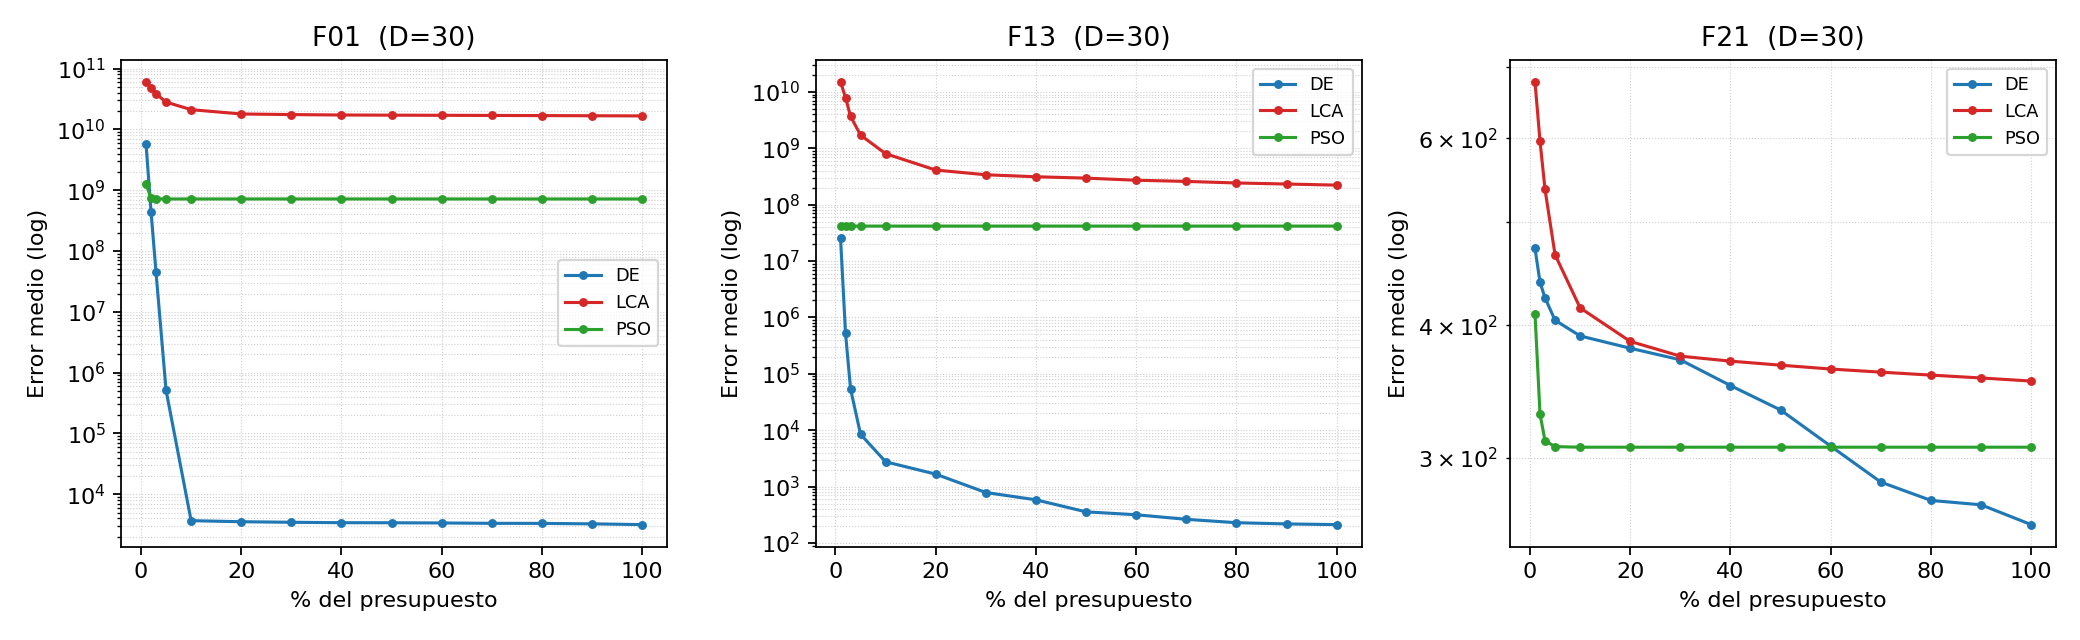
\includegraphics[width=\textwidth]{figuras/conv_ref.png}
\caption{Curvas de convergencia del error medio (escala log.) en $D=30$ para DE, LCA y PSO
sobre F1 (unimodal), F13 (híbrida) y F21 (compuesta). El LCA (rojo) se estanca pronto en un
error elevado, mientras DE refina varios órdenes de magnitud.}
\label{fig:conv_ref}
\end{figure}

\paragraph{Lectura de las curvas.}
En F1 el contraste es máximo: DE desciende más de seis órdenes de magnitud mientras el LCA se
estabiliza en torno a $10^{10}$ desde las primeras evaluaciones, sin progreso posterior. En la
híbrida F13 el LCA apenas progresa y se mantiene en la parte alta mientras DE domina. Solo en la compuesta
F21 ---donde todos los algoritmos rinden de forma parecida por la dificultad intrínseca de la
función--- las curvas se aproximan. El estancamiento temprano del LCA es, por tanto,
estructural y no un problema de presupuesto: ampliar las evaluaciones no mejoraría el
resultado.

\subsection{Validación en el problema del Portfolio (Prácticas 1--3)}
\label{sec:portfolio}

Para satisfacer la comparación explícita con las Prácticas~1--3, se ha adaptado el
LCA al problema de \textbf{optimización de carteras (Portfolio de Markowitz)} que
constituye el hilo conductor de la asignatura. La implementación reutiliza el
mismo marco de las prácticas ---la clase \texttt{PortfolioProblem}, con su función
de \emph{fitness} ($\text{beneficio}-\lambda\cdot\sigma$, donde $\sigma$ es la
desviación típica de la cartera) y su operador de reparación \texttt{fix()}--- de
modo que la comparación es directa y justa. El LCA conserva sus operadores
(crecimiento hemi-elipsoidal, vuelo de Lévy y metástasis), aplicando \texttt{fix()}
tras la inicialización y tras cada candidato para respetar las restricciones del
problema (pesos en rango, suma unitaria y cardinalidad). El protocolo replica
exactamente el de las prácticas: \textbf{50 ejecuciones}, $10\,000$ evaluaciones,
$\lambda=500$ y semilla base~42, sobre los tres mercados (IBEX~35, S\&P~100 y
S\&P~500). El problema se \emph{maximiza}, igual que en las prácticas; como el
término de riesgo es la desviación típica, los valores de \emph{fitness} son
negativos y \emph{mayor} (menos negativo) es mejor.

El Cuadro~\ref{tab:portfolio} recoge el \emph{fitness} medio de entrenamiento
(2015--2024)\footnote{Siguiendo la metodología de las Prácticas~2 y~3, los datos se
dividen temporalmente: la \emph{fase de búsqueda} (optimización) se realiza sobre el
periodo 2015--2024 y la \emph{fase de prueba} (validación) sobre 2025, para todos los
algoritmos. El \emph{fitness} de entrenamiento que aquí se reporta corresponde a la
fase de búsqueda; el año 2025 se reserva como conjunto de validación fuera de muestra.}
del LCA frente a una selección representativa de los algoritmos de las
Prácticas~1--3, \textbf{todos reejecutados bajo idénticas condiciones} y el mismo
marco experimental (Búsqueda Local y variantes de la P1; Algoritmo Genético,
Memético y Evolución Diferencial de la P2; Enfriamiento Simulado, BMB, ILS e
ILS-ES de la P3).

\begin{table}[h!]
\centering
\caption{Comparación en el problema del Portfolio: \emph{fitness} medio de
entrenamiento (2015--2024; mayor es mejor) sobre 50 ejecuciones. El LCA se compara
con los algoritmos de las Prácticas~1--3 reejecutados bajo el mismo marco
($\lambda=500$, $10\,000$ evals, semilla~42, fórmula con desviación típica). En
negrita el mejor por mercado.}
\label{tab:portfolio}
\begin{tabular}{lccc}
\toprule
Algoritmo & IBEX 35 & S\&P 100 & S\&P 500 \\
\midrule
Greedy (determinista, P1)        & -4.794 & -3.305 & -3.370 \\
Random (P1)                      & -4.911 & -3.400 & -3.648 \\
BL (P1)                          & -4.614 & -3.116 & -3.428 \\
BL Multiarranque (P1)            & -4.564 & -3.044 & -3.385 \\
Genético AGG-BLX (P2)            & -4.497 & -2.891 & -2.805 \\
Memético AM-Best (P2)            & \textbf{-4.490} & -2.816 & -2.735 \\
Evolución Diferencial (P2)       & -4.491 & \textbf{-2.807} & \textbf{-2.717} \\
Enfriamiento Simulado (P3)       & -4.653 & -3.300 & -4.062 \\
BMB (P3)                         & -4.574 & -3.006 & -3.263 \\
ILS (P3)                         & -4.606 & -3.114 & -3.434 \\
ILS-ES (P3)                      & -4.649 & -3.311 & -4.035 \\
\textbf{LCA (este trabajo)}      & \textit{-4.580} & \textit{-2.994} & \textit{-3.011} \\
\bottomrule
\end{tabular}
\end{table}

El resultado es revelador y matiza el comportamiento del LCA. En el Portfolio el
LCA queda en una \textbf{posición media de la tabla}: en S\&P~100 y S\&P~500 es el
\textbf{cuarto mejor} algoritmo ---solo por detrás del trío puntero formado por la
Evolución Diferencial, el Memético y el Genético BLX--- y en IBEX~35 se sitúa en la
zona media. De forma consistente en los tres mercados, el LCA \textbf{supera con
claridad a la Búsqueda Local y sus variantes (BL, BL~Multi), a la búsqueda aleatoria
y al Greedy}, e incluso bate a los métodos de trayectoria de la Práctica~3
(Enfriamiento Simulado, ILS, ILS-ES, BMB), que a este presupuesto de $10\,000$
evaluaciones convergen prematuramente. Sin embargo, \textbf{no alcanza a los
algoritmos poblacionales más potentes} (DE, Memético y Genético), que explotan
mejor las regiones prometedoras. Este resultado es \emph{más favorable} al LCA que
el obtenido en CEC2017 ---donde quedaba último--- pero sigue confirmando el mismo
diagnóstico: el LCA es un buen \emph{explorador} (bate a toda la familia de búsqueda
local y trayectoria) pero un \emph{explotador} mediocre frente a DE o a los
meméticos. La idoneidad relativa mejora en el Portfolio porque la dimensionalidad es
baja y el operador \texttt{fix()} encauza las soluciones hacia regiones factibles,
de modo que el vuelo de Lévy resulta efectivo; aun así, la brecha frente a los
mejores poblacionales vuelve a señalar la \textbf{explotación local} como el cuello
de botella, refrendando la hibridación memética de la Parte~III. Esto confirma
empíricamente que \emph{la idoneidad de una metaheurística es dependiente del
problema}, una de las conclusiones teóricas que persigue la práctica.

\subsection{Comparación con el estado del arte mediante Tacolab}
\label{sec:tacolab}

Además del análisis local frente a DE y PSO, se ha realizado una comparación
directa contra el \textbf{estado del arte del benchmark CEC2017} empleando la
herramienta \texttt{tacolab.org} \cite{tacolab}. Para ello se exportaron los
resultados del LCA y del LCA-SW (Parte~III) al formato de TACO y se enfrentaron,
en dimensión $D=30$ y al 100\% del presupuesto, a seis algoritmos de referencia
disponibles en su repositorio: \textbf{EBOwithCMAR} (ganador de la competición
CEC2017), \textbf{jSO}, \textbf{DE}, \textbf{PSO}, \textbf{SSA} (Salp Swarm
Algorithm) y \textbf{AEO} (Artificial Ecosystem-based Optimization), estos dos
últimos bioinspirados recientes de la misma familia que el LCA.

El Cuadro~\ref{tab:tacolab_rank} muestra el ranking medio de Friedman resultante
(menor es mejor). El LCA base queda \emph{último} entre los ocho algoritmos,
confirmando a gran escala lo ya observado frente a DE/PSO. La hibridación
memética, en cambio, eleva al \textbf{LCA-SW hasta la cuarta posición}, superando
a PSO, SSA y AEO, y situándose solo por detrás del trío puntero (DE, jSO,
EBOwithCMAR).

\begin{table}[h!]
\centering
\caption{Ranking medio de Friedman ($D=30$, 100\% del presupuesto, 30 funciones)
obtenido con Tacolab. Comparación conjunta del LCA y el LCA-SW frente a seis
algoritmos de referencia de CEC2017. Menor es mejor.}
\label{tab:tacolab_rank}
\begin{tabular}{clc}
\toprule
Posición & Algoritmo & Ranking medio \\
\midrule
1 & EBOwithCMAR (ganador CEC2017) & 1.583 \\
2 & jSO                           & 1.633 \\
3 & DE                            & 3.383 \\
4 & \textbf{LCA-SW (este trabajo)}& \textbf{4.200} \\
5 & PSO                           & 5.950 \\
6 & SSA                           & 6.017 \\
7 & AEO                           & 6.567 \\
8 & \textbf{LCA (este trabajo)}   & \textbf{6.667} \\
\bottomrule
\end{tabular}
\end{table}

El test de Wilcoxon por pares de Tacolab corrobora la lectura: el LCA base es
significativamente peor que todos los rivales salvo AEO ($p$-valores
$<0.05$), mientras que el LCA-SW \emph{gana de forma significativa} a AEO, PSO y
SSA ($p<0.01$) y solo cede frente a los DE-variants punteros (DE, jSO,
EBOwithCMAR). Esto sitúa la aportación de este trabajo ---el LCA hibridado--- en
la zona media-alta del estado del arte, un resultado notable para una
metaheurística que, en su forma original, partía de la última posición.

\subsection{Discusión de los resultados}

\paragraph{El LCA base no es competitivo frente a DE y PSO.}
El estudio multidimensional con 31 ejecuciones revela de forma inequívoca que el LCA base,
en su formulación original, queda por debajo de dos metaheurísticas clásicas bien
afinadas. La diferencia es estadísticamente significativa en las tres dimensiones. Lejos de
ser un resultado negativo, esto es coherente con la naturaleza de muchas metaheurísticas
bioinspiradas recientes: aportan mecanismos novedosos pero no necesariamente superan a
algoritmos consolidados como DE sin un ajuste fino o una hibridación. El propio enunciado de
la práctica advierte de que «la naturaleza de la MHe condicionará la calidad del resultado».

\paragraph{Debilidad principal: explotación local deficiente.}
La carencia más grave del LCA se observa en las funciones unimodales (F1, F3) y, en general,
en todas las dimensiones: errores de orden $10^{9}$--$10^{10}$ en F1 frente al $0$ o valores
moderados de DE. El operador de crecimiento adaptativo (volumen del hemi-elipsoide) genera
desplazamientos demasiado groseros para afinar sobre pendientes suaves, y el vuelo de Lévy,
aunque favorece la exploración, no compensa la falta de un refinamiento local preciso. Esta
debilidad estructural es la que justifica directamente la \textbf{hibridación memética con
Solis-Wets} de la Parte~III.

\paragraph{Comparación con las prácticas anteriores.}
El guion exige comparar la MHe con los resultados de las Prácticas~1--3. Estas
abordan un problema distinto ---la optimización de carteras de inversión
(\emph{Portfolio} de Markowitz sobre IBEX/S\&P)--- por lo que no producen
resultados sobre CEC2017. La comparación se ha resuelto por \textbf{dos vías
complementarias}: (i) en el propio benchmark CEC2017, enfrentando el LCA a DE y
PSO bajo idéntico protocolo y, además, al estado del arte vía Tacolab
(Sección~\ref{sec:tacolab}); y (ii) llevando el LCA al \textbf{problema del
Portfolio de las prácticas} y comparándolo, bajo el mismo marco experimental, con
los algoritmos efectivamente desarrollados en las Prácticas~1, 2 y~3 ---Búsqueda
Local y variantes, Algoritmo Genético, Memético, Evolución Diferencial,
Enfriamiento Simulado, BMB, ILS e ILS-ES--- todos reejecutados a $\lambda=500$,
$10\,000$ evaluaciones y semilla~42 (Sección~\ref{sec:portfolio}). El contraste
entre ambos escenarios resulta revelador: un LCA \emph{último} en CEC2017 asciende
a la \emph{zona media} en el Portfolio, donde supera a toda la familia de búsqueda
local y de trayectoria pero sigue por debajo de los poblacionales punteros
(DE, Memético, Genético). Ambos escenarios convergen en el mismo diagnóstico ---el
LCA explora bien pero explota mal--- lo que confirma que la calidad de una
metaheurística depende fuertemente del problema y refuerza la necesidad de la
hibridación local desarrollada en las Partes~III y~IV.

